\documentclass{beamer}
\usetheme{Madrid}
\usecolortheme{seahorse}
\usepackage{graphicx} % Required for inserting images
\usepackage{amsfonts}
\usepackage{amsmath}
\usepackage{amssymb}
\usepackage{subcaption}
\usepackage{animate}
\usepackage{natbib}
\bibliographystyle{apalike}
\usepackage[portuguese]{babel}
\usepackage{indentfirst}

\title{O Método dos Elementos Virtuais em elastodinâmica}
\author{Vinícius B. A. P. Pohl \inst{1}}
\date{Agosto de 2026}
\logo{
\includegraphics[width=0.2\linewidth]{figuras/ppgmne jpge 2 (1).png}}

\institute[UFPR] % (optional)
{
  \inst{1}%
  Programa de Pós-graduação em Métodos Numéricos em Engenharia\\
  Universidade Federal do Paraná
}

\begin{document}

\frame{\titlepage}

\begin{frame}
    \frametitle{Table of Contents}
    \tableofcontents
\end{frame}

\section{Introdução}

\begin{frame}{O método dos elementos virtuais}
    \begin{itemize}
        \item Técnica de solução de EDPs com valores de contorno através da partição do domínio
        \item Elementos de geometria arbitrária \pause 
        \item Funções de base desconhecidas
    \end{itemize} 
    \begin{figure}
            \centering
            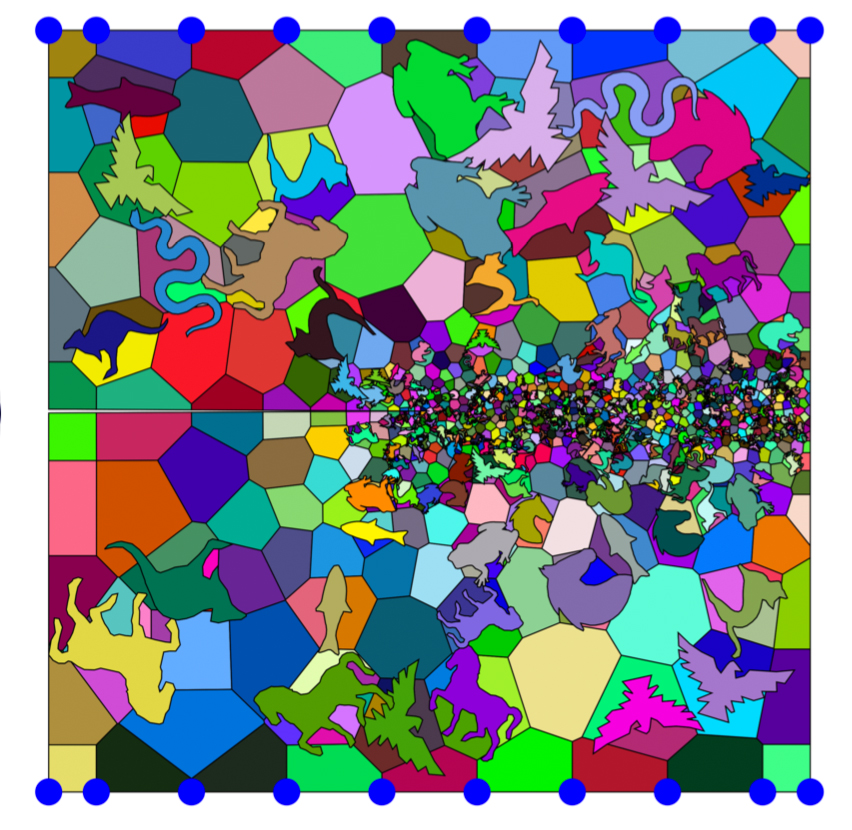
\includegraphics[width=0.4\linewidth]{figuras/voronoi_mesh.png}
        \end{figure}
        {\centering Fonte: \cite{virtualelementformulationphasefieldmodelingductilefracture2019}}
\end{frame}

\begin{frame}{Desenvolvimento do método}
    \begin{enumerate}
        \item Desenvolvido a partir da técnica de Diferenças Finitas Miméticas
        \item Artigo fundacional: \cite{basicprinciplesvirtualelementmethods2013a}
        \item Problemas vetoriais: \cite{virtualelementslinearelasticityproblems2013}
        \item Extensão para $C^\alpha$: \cite{virtualelementmethodarbitraryregularity2014}
        \item Espaço de funções ampliado: \cite{equivalentprojectorsvirtualelementmethods2013a}
        \item Espaços $H(div)$ e $H(rot)$: \cite{hdivhcurlconformingvem2014}
    \end{enumerate}
\end{frame}

\section{O problema discreto}

\begin{frame}{Equação diferencial da elastodinâmica}
    \indent Problemas elastodinâmicos são regidos pela equação: $$\begin{aligned}
        \rho \ddot{u} - \nabla \cdot \sigma(u)  = f \hspace{0.5cm} \text{in} \hspace{3mm} \Omega \times (0,T],  \\
        u = g_D \hspace{0.5cm} \text{in} \hspace{3mm} \Gamma_D \times (0,T],\\
        \sigma (u) n = g_N \hspace{0.5cm} \text{in} \hspace{3mm} \Gamma_N \times (0,T],\\
        u = u_0 \hspace{0.5cm} \text{in} \hspace{3mm} \Omega \times \{0\},\\
        \dot{u} = u_1 \hspace{0.5cm} \text{in} \hspace{3mm} \Omega \times \{0\}.
    \end{aligned}$$
\end{frame}

\begin{frame}{Forma variacional}
    As matrizes de elementos virtuais são construídas utilizando a forma variacional.\\
    A forma variacional é obtida do Método de Galerkin ou pela minimização do funcional de energia. O problema na forma bilinear é: $$m(\ddot{u_h},v_h) + c(\dot{u_h},v_h) + a(u_h,v_h) = \left<f_h,v_h\right>. $$
    Ou na forma matricial discreta:
    $$[ M ] \ddot{u} + [C]\dot{u} + [K]u = f.$$\pause
    Em problemas de vibração livre a equação se simplifica para: $$[M] \ddot{u} + [K]u = 0.$$
\end{frame}

\begin{frame}{O problema de autovalores}
    As frequências naturais provém da solução do problema de autovalor: $$\left([K]-\omega^2[M]\right)\phi_ = 0,$$ com $$\begin{aligned} [M] = \int_E \rho \, \varphi^T\varphi dE \\ [K] = \int_E \epsilon(\varphi)^T \mathbb{C} \epsilon(\varphi)  dE. \end{aligned}$$
\end{frame}

\section{O Método dos Elementos Virtuais}

\subsection{Propriedades e bases}

\begin{frame}{Espaços de aproximação}
    Para definir o espaço de aproximação do método, primeiro define-se um espaço auxiliar: $$\mathbb{B}_k(\partial E) := \{ v \in C^0(\partial E) : v_{|e} \in \mathbb{P}_k(e) \forall e \subset \partial E \}.$$ \pause
    O espaço de aproximação é dado por: $$V^{\Omega,k}:=\{v \in H^1(\Omega): v_{|\partial\Omega} \in \mathbb{B}_k(\partial\Omega), \nabla^2 v_{\Omega} \in \mathbb{P}_{k-2}(\Omega)\}.$$ \pause 
    O espaço ampliado de \cite{equivalentprojectorsvirtualelementmethods2013a} é:$$\begin{aligned}
        \mathbb{V}^{E,k}:=\{v_h \in H^1(\Omega): v_{|\partial E} \in \mathbb{B}_k(\partial E), \nabla^2 v_{\Omega} \in \mathbb{P}_{k}(E), \\ \int_E (v_h - \Pi_k^\nabla v_h) \mu_h dE \hspace{2mm} \forall\mu_h \in \mathbb{P}_k(E)\backslash \mathbb{P}_{k-2}(E) \}.
    \end{aligned}$$
\end{frame}

\begin{frame}{Propriedades do método}
    \begin{enumerate}
        \item K-consistência: Para todo $p \in \mathbb{P}_k(\Omega)$ e para todo $v_h \in V_{h|\Omega}$,  $$a^K(p,v_h) = a_h^K(p,v_h)$$
        \item Estabilidade: Existem duas constantes positivas $\alpha_*$ e $\alpha^*$, independentes de $h$ e de $\Omega$, tal que $$\forall v_h \in \mathbb{V}^{E,k}_h, \hspace{3mm} \alpha_* a^K(v_h,v_h) \leq a_h^K((v_h,v_h) \leq \alpha^* a^K(v_h,v_h)$$
    \end{enumerate}    
\end{frame}

\begin{frame}{bases}
    Uma das partes mais importantes do método é a escolha da base polinomial a ser utilizada.\\
    Uma escolha comum é: $$p_{\alpha} = \left(\frac{x -\bar{x}}{h_E}\right)^{\alpha_1}\left(\frac{y -\bar{y}}{h_E}\right)^{\alpha_2}$$ \pause
    As bases forma um conjunto polinomial $p_\alpha \in \mathbb{P}_k(\Omega)$. 
\end{frame}

\begin{frame}{Projeção}
    As funções de base são desconhecidas, mas o espaço de aproximação é mapeado através de um operador de projeção:$$\Pi_k : V^{\Omega,k} \rightarrow \left[\mathbb{P}_k(\Omega)\right]^2$$. \pause
    As funções de base podem ser divididas em dois termos:$$\varphi=\Pi_k\varphi + (I -\Pi_k)\varphi.$$ 
\end{frame}

\begin{frame}{Subdivisão da forma bilinear}
    Assim como há a subdivisão das funções de base, também há das formas bilineares. $$\begin{aligned}
        m_{\Omega_v}(\ddot{u_h},v_h) = m_{\Omega_v}(\Pi\ddot{u_h},\Pi v_h) + \tau_h S_{\Omega_v}(\ddot{u_h},v_h) \\
        a(u_h,v_h) = a_{\Omega_v}(\Pi u_h,\Pi v_h) + \tau_h S_{\Omega_v}(u_h,v_h)
    \end{aligned}$$
\end{frame}

\begin{frame}{funções de base}
    As funções de base são definidas iguais a base canônica.\\
    Para um operador $\chi_i$ relativo aos graus de liberdade: $$\chi_i(\varphi_j) = \delta_{ij}$$.
    As funções de base apresentam a identidade tipo Lagrangeana:
    $$u_h = \{\varphi\}^T \{u_h^E\}$$ \pause
    O projetor é construído em cima da base polinomial:$$\Pi_k u_h = \{p_\alpha\}^T \{a\}$$
\end{frame}

\subsection{O elemento virtual}

\begin{frame}{Elemento virtual}
    \begin{figure}
        \centering
        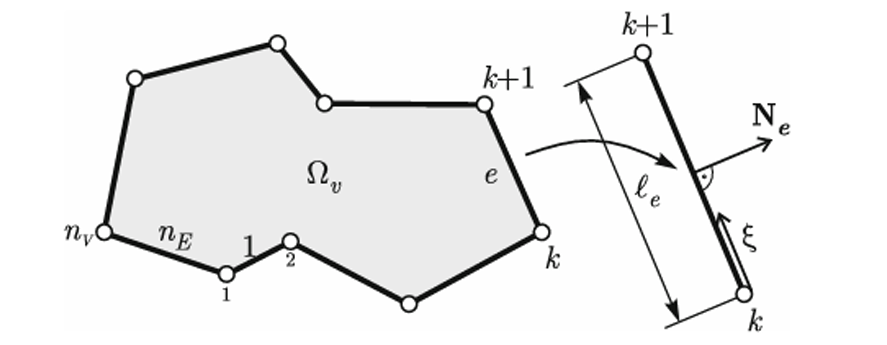
\includegraphics[width=0.5\linewidth]{figuras/Elemento.png}
    \end{figure} 
    {\centering{\small Fonte: \cite{virtualelementmethodsengineeringsciences2024}}}\\[5mm] \pause 
    Os graus de liberdade são:
    \begin{itemize}
        \item Vértices: $n_v$
        \item Arestas: $n_v(k-1)$
        \item internos: $\frac{k(k - 1)}{2}$
    \end{itemize}
\end{frame}

\begin{frame}{Momentos internos}
    A quantidade de momentos internos equivale à dimensão de um polinômio $k-2$. Os momentos internos são: $$m = \frac{1}{|E|}\int_{E} p_{\alpha} v_h, \hspace{2mm} \alpha = 1,\ldots,n_{k-2}.$$ \pause
    A relação entre o grau de aproximação é:
    \begin{figure}
        \centering
        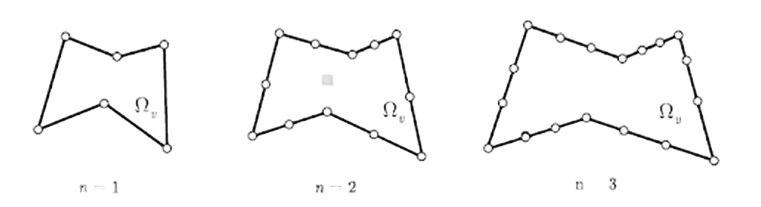
\includegraphics[width=1.0\linewidth]{figuras/gdl (1).png}
    \end{figure}
\end{frame}

\subsection{Consistência}

\begin{frame}{O projetor $H^1$}
    Para o calculo do projetor, a seguinte equação deve ser satisfeita: $$\begin{cases}
        b^E(\Pi^\nabla_k v_h,q) = b^E(v_h,q) \hspace{2mm} \forall q\in \mathbb{P}_k(E) \\
        \bar{\Pi_k^\nabla v_h} = \bar{v_h},
    \end{cases}\hspace{3mm} \forall v_h \in \mathbb{V}^{E,k}$$ \pause \\
    A primeira equação em formato matricial:
    $$\mathcal{G}^\nabla \Pi_k^\nabla = \mathcal{B}^\nabla$$
\end{frame}

\begin{frame}{Matriz $\mathcal{B}^\nabla$}
    A parcela não é computável. Aplica-se o teorema da divergência:
    $$\mathcal{B}^\nabla = \int_{\Gamma_e} (\nabla q \cdot n) v_{h|\Gamma_e} - \int_E \nabla^2(q) v_h$$ \pause
    Parcela de contorno pode ser aproximada por quadratura:
    $$\mathcal{B}^\nabla(v_h,m_i) = \sum_{j=1}^{n_e} l_e\sum_{r=1}^{k+1} w_r \nabla \left(q(\xi_j,\eta_j)\right) n - \nabla^2 \left(q(\xi,\eta)\right) \{m_i\} $$
\end{frame}

\begin{frame}{Matriz $\mathcal{G}^\nabla$}
    A matriz $\mathcal{G}^\nabla$ pode ser computada das seguintes maneiras:
    \begin{enumerate}
        \item Quadratura numérica;
        \item integração exata por momentos arbitrários;
        \item identidade: $\mathcal{G} = \mathcal{B}\mathcal{D}$
    \end{enumerate}
\end{frame}

\begin{frame}{Matriz $\mathcal{D}^\nabla$}
    \begin{enumerate}
        \item Matriz de mudança de base. Polinomial $\rightarrow$ Canônica
        \item $D_{i\alpha} = \chi_i(p_\alpha)$
    \end{enumerate}
\end{frame}

\begin{frame}{Projetor $L^2$}
    \begin{enumerate}
        \item Utilizado nas matrizes de carga e de massa;
        \item não contém operadores diferenciais;
        \item necessário uso do espaço ampliado. 
    \end{enumerate} \pause
    $$\int_E \Pi_k^0 v_h q = \int_E v_h q \Leftrightarrow \mathcal{H} \Pi_k^0 = \mathcal{C}$$ \pause 
    \begin{enumerate}
        \item $\mathcal{H}$ obtida de integração numérica ou exata;
        \item Matriz $\mathcal{C}$ é:
    \end{enumerate}
    $$\mathcal{C}_{\alpha} = \begin{cases}
        (v_h,p_\alpha)_E \hspace{3mm} \text{se} \hspace{2mm} 1 \leq \alpha \leq n_{k-2} \\
        (\Pi_k^\nabla v_h,p_\alpha)_E \hspace{3mm} \text{se} \hspace{2mm} n_{k-2}+1 \leq \alpha \leq n_{k}
    \end{cases}$$
\end{frame}

\begin{frame}{Projetor de deformações}
    \begin{itemize}
        \item Formulação mais nova
        \item aproxima o campo de deformações diretamente
        \item $\Pi_{k-1}: \mathbb{V}^{E,k} \rightarrow \left[\mathbb{P}_{k-1}(E)\right]^3$
    \end{itemize}\pause
    A seguinte relação deve ser satisfeita:
    $$(\Pi^0_{k-1} \epsilon(v_h),q)_E = (\epsilon(v_h),q)_E \hspace{2mm} \forall q\in \left[\mathbb{P}_{k-1}(E)\right]^3$$
    Nessa formulação $\epsilon(v_h)$ é uma variável e aproximada diretamente. Matricialmente:
    $$\mathcal{G}^\epsilon \Pi_{k-1}^0 = \mathcal{B}^\epsilon$$
\end{frame}

\begin{frame}{Projetor de deformações}
    \begin{enumerate}
        \item $\mathcal{G}^\epsilon$ é integrada numericamente ou por integração direta
        \item $\mathcal{B}^\epsilon$ adota-se procedimento similar ao projetor $\Pi_k^\nabla$: $$\mathcal{B}^\epsilon(v_h,m_i) = \sum_{j=1}^{n_e} l_e\sum_{r=1}^{k+1} w_r \left(q(\xi_j,\eta_j)\right) n - \nabla \cdot \left(q(\xi,\eta)\right) \{m_i\}$$
    \end{enumerate}
\end{frame}

\subsection{Estabilização}

\begin{frame}{Métodos de estabilização}
    Diversas técnicas foram propostas na literatura para estabilização:
    \begin{itemize}
        \item \cite{basicprinciplesvirtualelementmethods2013a}: $$S_E = (I - D\Pi_k)^T(I - D\Pi_k);$$
        \item \cite{arbitraryorder2dvirtualelementspolygonalmeshespartelasticproblem2017a}: $$S_E = \left[I - D(D^TD)^{-1}D^T \right];$$
        \item \cite{wriggers2017efficient}: $$U_{stab} = \sum_{v=1}^{n_v}\int_E \bar{\psi}(u_h)dE + \sum_{v=1}^{n_v}\int_E \bar{\psi}(\Pi_k u_h)dE$$
    \end{itemize}    
\end{frame}

\begin{frame}{Parâmetros de estabilização}
    Os parâmetros são diversos. Aqui utiliza-se o parâmetro de \cite{numericalrecipeselastodynamicvirtualelementmethodsexplicittimeintegration2020}: $$\begin{aligned}
        \tau_k = \text{max}\left(\frac{tr(K^{c})}{n_{dof}}, \alpha_0 \frac{\mathbb{C}}{3}\right)\\
        \tau_m = \rho |E|
    \end{aligned}$$
\end{frame}

\section{Testes numéricos}

\begin{frame}{Problema proposto}
    Aqui se propõe uma viga em balanço:
    \begin{figure}
        \centering
        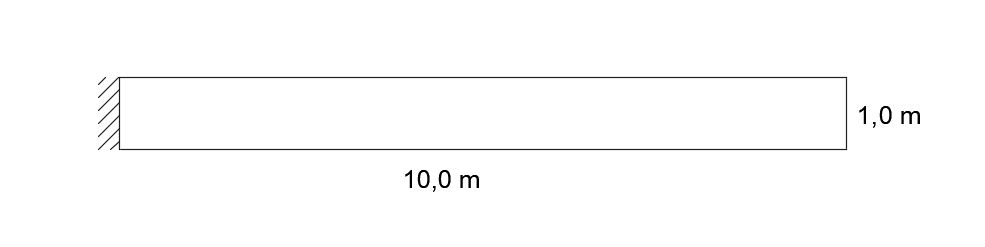
\includegraphics[width=1.0\linewidth]{figuras/Captura de tela 2026-08-27 104659.png}
    \end{figure}
    Diversos níveis de discretização são utilizados e compara-se os resultados do Método dos elementos virtuais (MEV) com os do método dos elementos finitos (MEF).
\end{frame}

\begin{frame}{Problema proposto}
    \begin{figure}
        \centering
        \begin{subfigure}[b]{0.48\textwidth}
            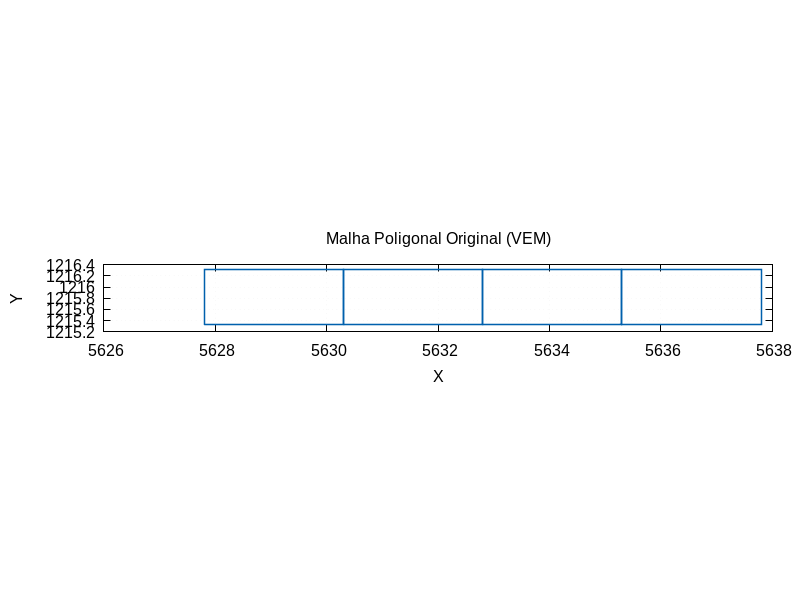
\includegraphics[width=0.9\linewidth]{figuras/M1.png}
        \end{subfigure}
        \hfill
        \begin{subfigure}[b]{0.48\textwidth}
            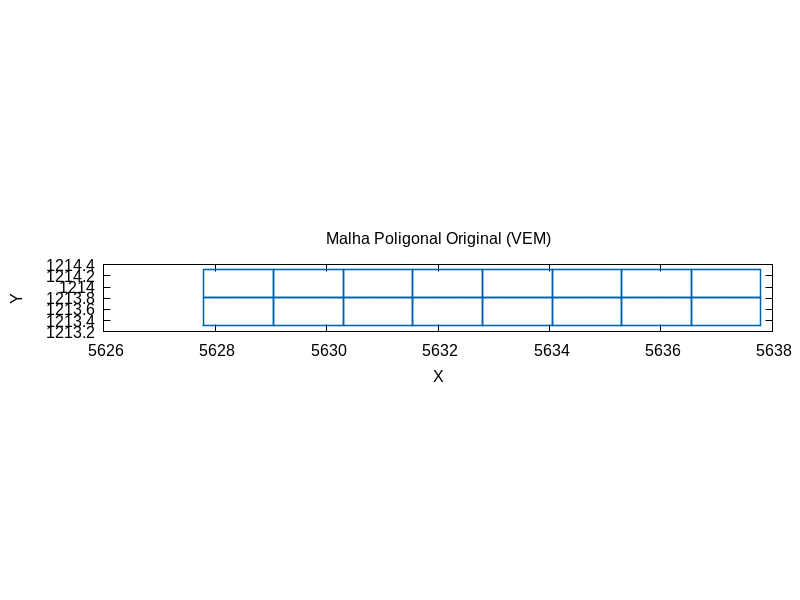
\includegraphics[width=0.9\linewidth]{figuras/M2.png}
        \end{subfigure}
        \begin{subfigure}[b]{0.48\textwidth}
            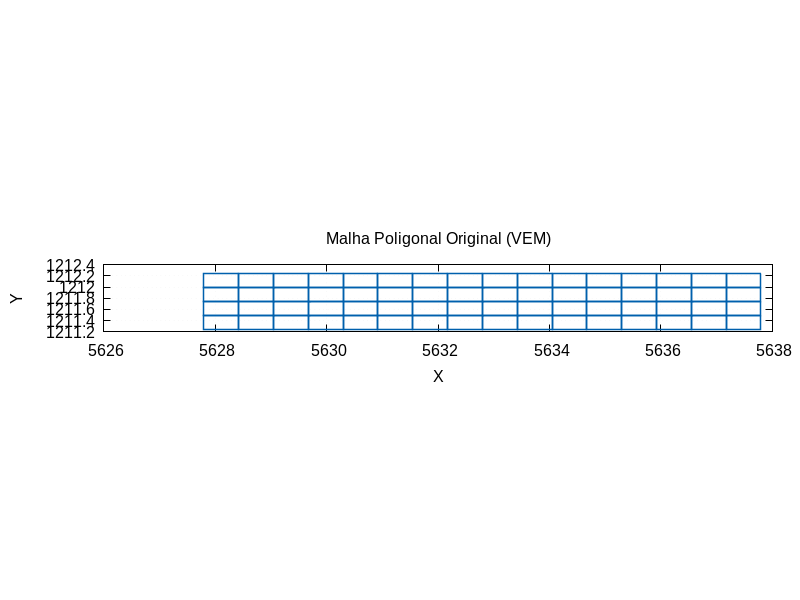
\includegraphics[width=0.9\linewidth]{figuras/M3.png}
        \end{subfigure}
    \end{figure}
\end{frame}

\begin{frame}{Aproximação $k=1$}
    \begin{figure}
        \centering
        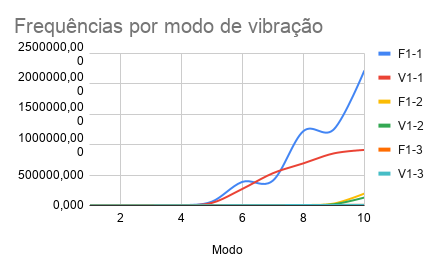
\includegraphics[width=1.0\linewidth]{figuras/Frequências por modo de vibração_1.png}
    \end{figure}
\end{frame}

\begin{frame}{Análise individual de frequências para cada malha}
    \begin{figure}
        \centering
        \begin{subfigure}[b]{0.48\textwidth}
            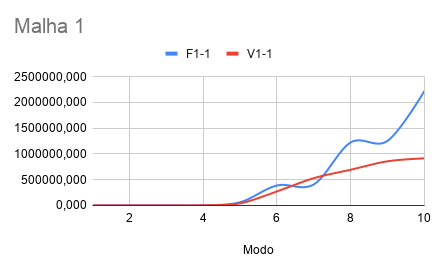
\includegraphics[width=0.9\linewidth]{figuras/Malha 1.png}
        \end{subfigure}
        \hfill
        \begin{subfigure}[b]{0.48\textwidth}
            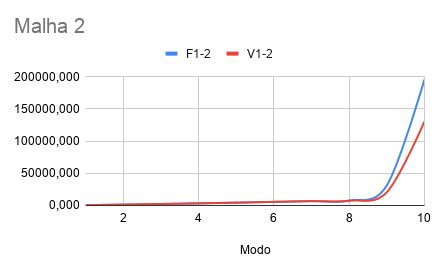
\includegraphics[width=0.9\linewidth]{figuras/Malha 2.png}
        \end{subfigure}
        \begin{subfigure}[b]{0.48\textwidth}
            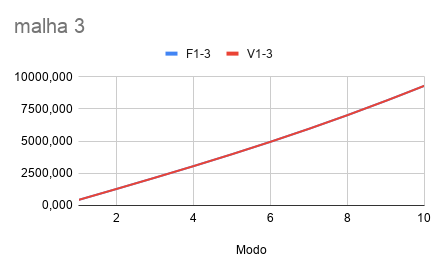
\includegraphics[width=0.9\linewidth]{figuras/malha 3.png}
        \end{subfigure}
    \end{figure}
\end{frame}

\begin{frame}{Aproximação $k=2$}
    \begin{figure}
        \centering
        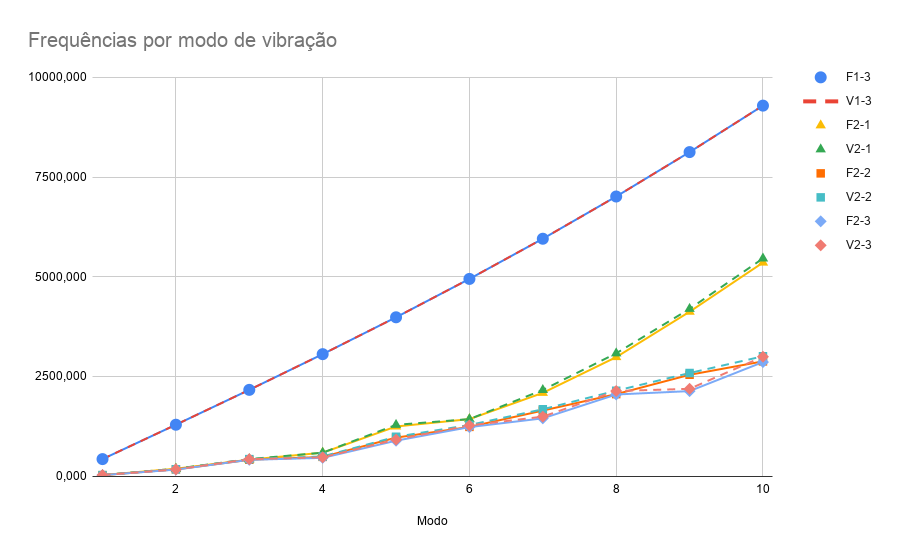
\includegraphics[width=1.0\linewidth]{figuras/Frequências por modo de vibração (2).png}
    \end{figure}
\end{frame}

\begin{frame}{Análise individual de frequências para cada malha com $k=2$}
    \begin{figure}
        \centering
        \begin{subfigure}[b]{0.48\textwidth}
            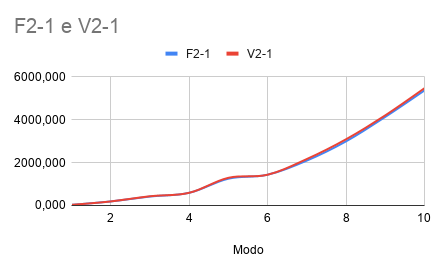
\includegraphics[width=0.9\linewidth]{figuras/F2-1 e V2-1.png}
        \end{subfigure}
        \hfill
        \begin{subfigure}[b]{0.48\textwidth}
            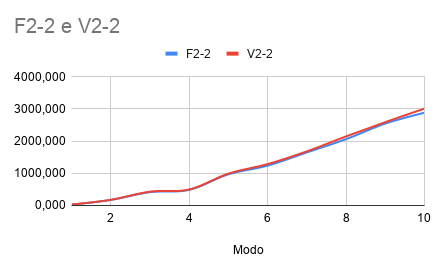
\includegraphics[width=0.9\linewidth]{figuras/F2-2 e V2-2.png}
        \end{subfigure}
        \begin{subfigure}[b]{0.48\textwidth}
            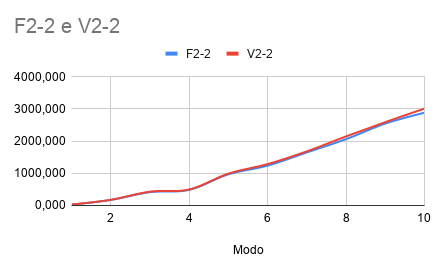
\includegraphics[width=0.9\linewidth]{figuras/F2-2 e V2-2.png}
        \end{subfigure}
    \end{figure}
\end{frame}

\begin{frame}{Erro do MEV}
    \begin{figure}
        \centering
        \begin{subfigure}[b]{0.48\textwidth}
            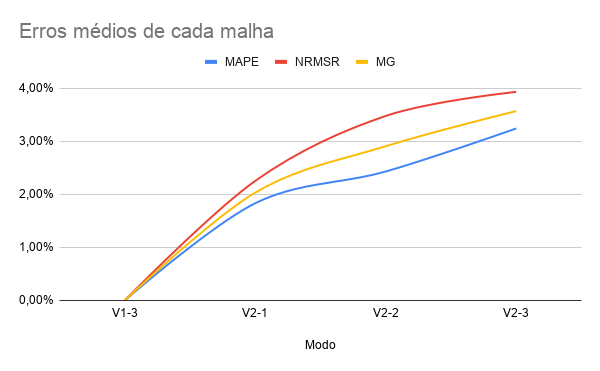
\includegraphics[width=1.0\linewidth]{figuras/Erros médios de cada malha.png}
        \end{subfigure}
        \hfill
        \begin{subfigure}[b]{0.48\textwidth}
            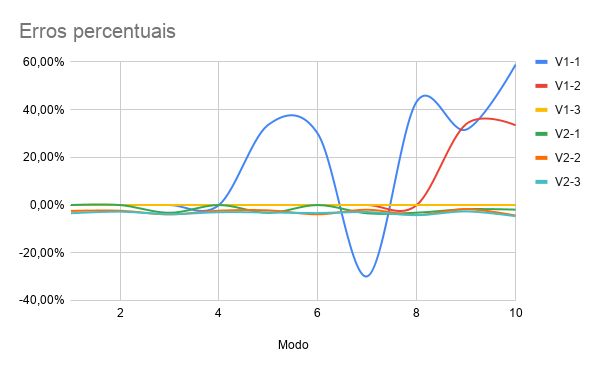
\includegraphics[width=1.0\linewidth]{figuras/Erros percentuais.png}
        \end{subfigure}
    \end{figure}
\end{frame}

\begin{frame}{Malhas deformadas}
    \begin{figure}
        \centering
        \begin{subfigure}[b]{1.0\textwidth}
            
\includegraphics[width=0.5\linewidth]{figuras/deformed_mode_1.png}
        \end{subfigure}
        \hfill
        \begin{subfigure}[b]{1.0\textwidth}
            
\includegraphics[width=0.5\linewidth]{figuras/deformed_mode_2.png}
        \end{subfigure}
    \end{figure}
    \begin{figure}
        \centering
        \begin{subfigure}[b]{1.0\textwidth}
            
\includegraphics[width=0.5\linewidth]{figuras/deformed_mode_3.png}
        \end{subfigure}
        \hfill
        \begin{subfigure}[b]{1.0\textwidth}
            
\includegraphics[width=0.5\linewidth]{figuras/deformed_mode_4.png}
        \end{subfigure}
    \end{figure}
\end{frame}

\begin{frame}{malhas deformadas}
    \animategraphics[loop, autoplay, every=1, width=1.0\textwidth]{12}{figuras/gif/frame_}{00}{39}
\end{frame}

\section{Referências}

\begin{frame}{Referências}
    \tiny
    \bibliography{Ref}
\end{frame}


\end{document}
